\subsection{Purpose}
The goal of this project is to design a game for two or more players, where the STM32’s microphone is used to control a robot.\\*
This project is a variant of the project proposal where the STM32F4 was used in a game for two or more players to choose and recognize a frequency with the microphone.\\*
In this project, the embedded microphone of the board is used to control the stepper motors and move the robot on the surrounding environment.

\subsection{Description of the robot}
The robot has a cylindrical shape and it is equipped with wheels on the bottom that allow it to move forward, backward, turn left and right.\\*
The structure of the project is divided in two different part: the transmitter and the receiver.
The transmitter is represented by the STM32F4 discovery board which is in charge to recognize the frequency of the sounds emitted by the player, elaborate them into commands and send these commands to the receiver.
The receiver is represented by an Arduino board which is directly connected to the mechanical body of the robot. The Arduino board receives the commands from the discovery board and uses them to control the engines of the robot.
The wireless communication is managed through two hc-05 Bluetooth modules: one for the transmitter and one for the receiver.
We used a 3D printer to build the body of the robot. 

\subsection{Game logic}
The game consists of a race between two or more robots. Each player controls his own robot through whistles, and he will guide it along the way. The most skilled player in the control of the robot, the one who will arrive first at the end of the path, will be the winner.\\*
A specific movement of the robot will correspond to each sound (frequency):
\begin{itemize}
	\item Forward movement
	\item Backward movement
	\item Left movement
	\item Right movement
\end{itemize}

\subsection{Code structure}
The code is structured in many components, in order to make the project extendable, easy to edit and easy to readapt.\\*
The main core of the project is represented by the transmitter. All other components of the robot are connected to the receiver.\\*
The frequency analyser converts the analog data obtained with the microphone into digital numbers.\\*
These information are translated in commands used to control the wheels of the robot.

\newpage
\begin{figure}[h!]
	\hspace*{-0.15 \textwidth}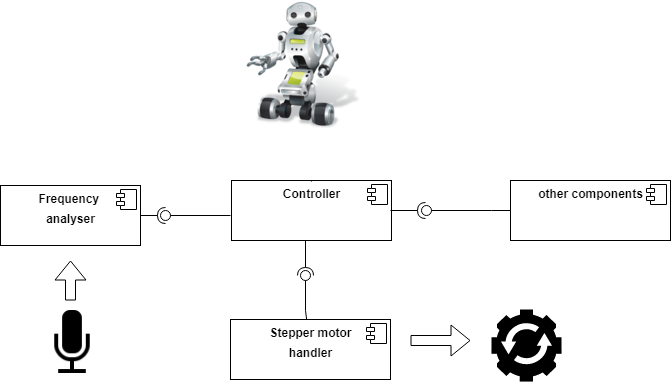
\includegraphics[width= 1.3\textwidth]
	{files/images/SystemStructure}
	\caption{This is a general overview of the system.}
\end{figure}